\documentclass[english,11pt,a4paper,titlepage]{report}
\usepackage[T1]{fontenc}
\usepackage{graphicx}
\usepackage{amsmath}
\usepackage{babel}
\usepackage{listings}
\title{Handin 2 - Neural Nets for Multiclass Classification}
\author{Rasmus Freund - 201700273}
\lstset{numbers=left,language=Python,frame=single,showtabs=false,breaklines=true,tabsize=4,xrightmargin=-20mm}
\begin{document}
	\maketitle
	
	\section*{Part I: Derivative}
	Given a one-hot-label vector $y$ with $y_j = 1$, show that:
	\begin{equation*}
	\frac{\partial L}{\partial z_i} = - \delta_{i,j} + \frac{1}{\sum_{a=1}^{k} e^{z_a}} \times e^{z_i} = -\delta_{i,j} + softmax(z)_i
	\end{equation*}
	where $\delta_{i,j} = 1$ if $i=j$ and zero otherwise.
	
	\subsubsection{Solution}
	Softmax is defined as:
	\begin{equation*}
	softmax(z)_i = \frac{e^{z_i}}{\sum_{a=1}^{k} e^{z_a}}
	\end{equation*}
	Therefore, the negative log-likelihood for the true class $j$ is:
	\begin{equation*}
	L(z) = -ln(softmax(z)_j) = -ln \left( \frac{e^{z_j}}{\sum_{a=1}^{k} e^{z_a}} \right)
	\end{equation*}
	The derivate of $L(z)$ w.r.t. $z_i$ when $i=j$ is then:
	
	\begin{equation*}
	\frac{\partial L}{\partial z_i} = -\frac{1}{softmax(z)_j} \times \frac{\partial softmax(z)_j}{\partial z_i}
	\end{equation*}
	Calculating the partial derivative of $softmax(z)_j$ w.r.t. $z_i$
	\begin{align*}
	\frac{\partial softmax(z)_j}{\partial z_i} &= \frac{\partial}{\partial z_i} \left( \frac{e^{z_i}}{\sum_{a=1}^{k} e^{z_a}} \right) \\[7pt]
											   &= \frac{e^{z_j \times \sum_{a=1}^{k} (e^{z_a})-e^{z_j} \times e^{z_i}}}{(\sum_{a=1}^{k} e^{z_a})^2} \\[7pt]
											   &= \frac{e^{z_j}}{\sum_{a=1}^{k} e^{z_a}} - \left( \frac{e^{z_j}}{\sum_{a=1}^{k} e^{z_a}} \right)^2 \\[7pt]
											   &= softmax(z)_j - (softmax(z)_j)^2
	\end{align*}
	Plugging this back into the original partial derivative
	\begin{align*}
	\frac{\partial L}{\partial z_i} &= -\frac{1}{softmax(z)_j} \times (softmax(z)_j - (softmax(z)_j)^2) \\
									&= -1 + softmax(z)_j
	\end{align*}
	Since $\delta_{i,j}=1$ if $i=j$
	\begin{equation*}
	\underline{\underline{\frac{\partial L}{\partial z_i} = -\delta_{i,j} + softmax(z)_i}}
	\end{equation*}
	
	\section*{Part II: Implementation and test}	
	
	\begin{lstlisting}
@staticmethod
def cost_grad(X, y, params, c=0.0):
	cost = 0
	W1 = params["W1"]
	b1 = params["b1"]
	W2 = params["W2"]
	b2 = params["b2"]
	d_w1 = None
	d_w2 = None
	d_b1 = None
	d_b2 = None
	labels = one_in_k_encoding(y, W2.shape[1])  # shape n x k
	
	### YOUR CODE HERE - FORWARD PASS
	# Number of samples
	n = X.shape[0]
	
	Z1 = X.dot(W1) + b1
	A1 = relu(Z1)
	Z2 = A1.dot(W2) + b2
	A2 = softmax(Z2)
	# Compute cost
	cost = -np.sum(labels * np.log(A2)) / n
	# Add regularization
	cost += c * (np.sum(W1 ** 2) + np.sum(W2 ** 2)) / (2 * n)
	### END CODE
	### YOUR CODE HERE - BACKWARDS PASS
	# Gradients of output
	d_Z2 = A2 - labels
	d_w2 = A1.T.dot(d_Z2) / n + c * W2 / n
	d_b2 = np.sum(d_Z2, axis=0, keepdims=True) / n
		
	d_A1 = d_Z2.dot(W2.T)
	d_Z1 = d_A1 * (Z1 > 0)  # RelU derivative
	d_w1 = X.T.dot(d_Z1) / n + c * W1 / n
	d_b1 = np.sum(d_Z1, axis=0, keepdims=True) / n
	### END CODE
	# the return signature
	return cost, {"d_w1": d_w1, "d_w2": d_w2, "d_b1": d_b1, "d_b2": d_b2}
	\end{lstlisting}

	\begin{figure}
		\centering
		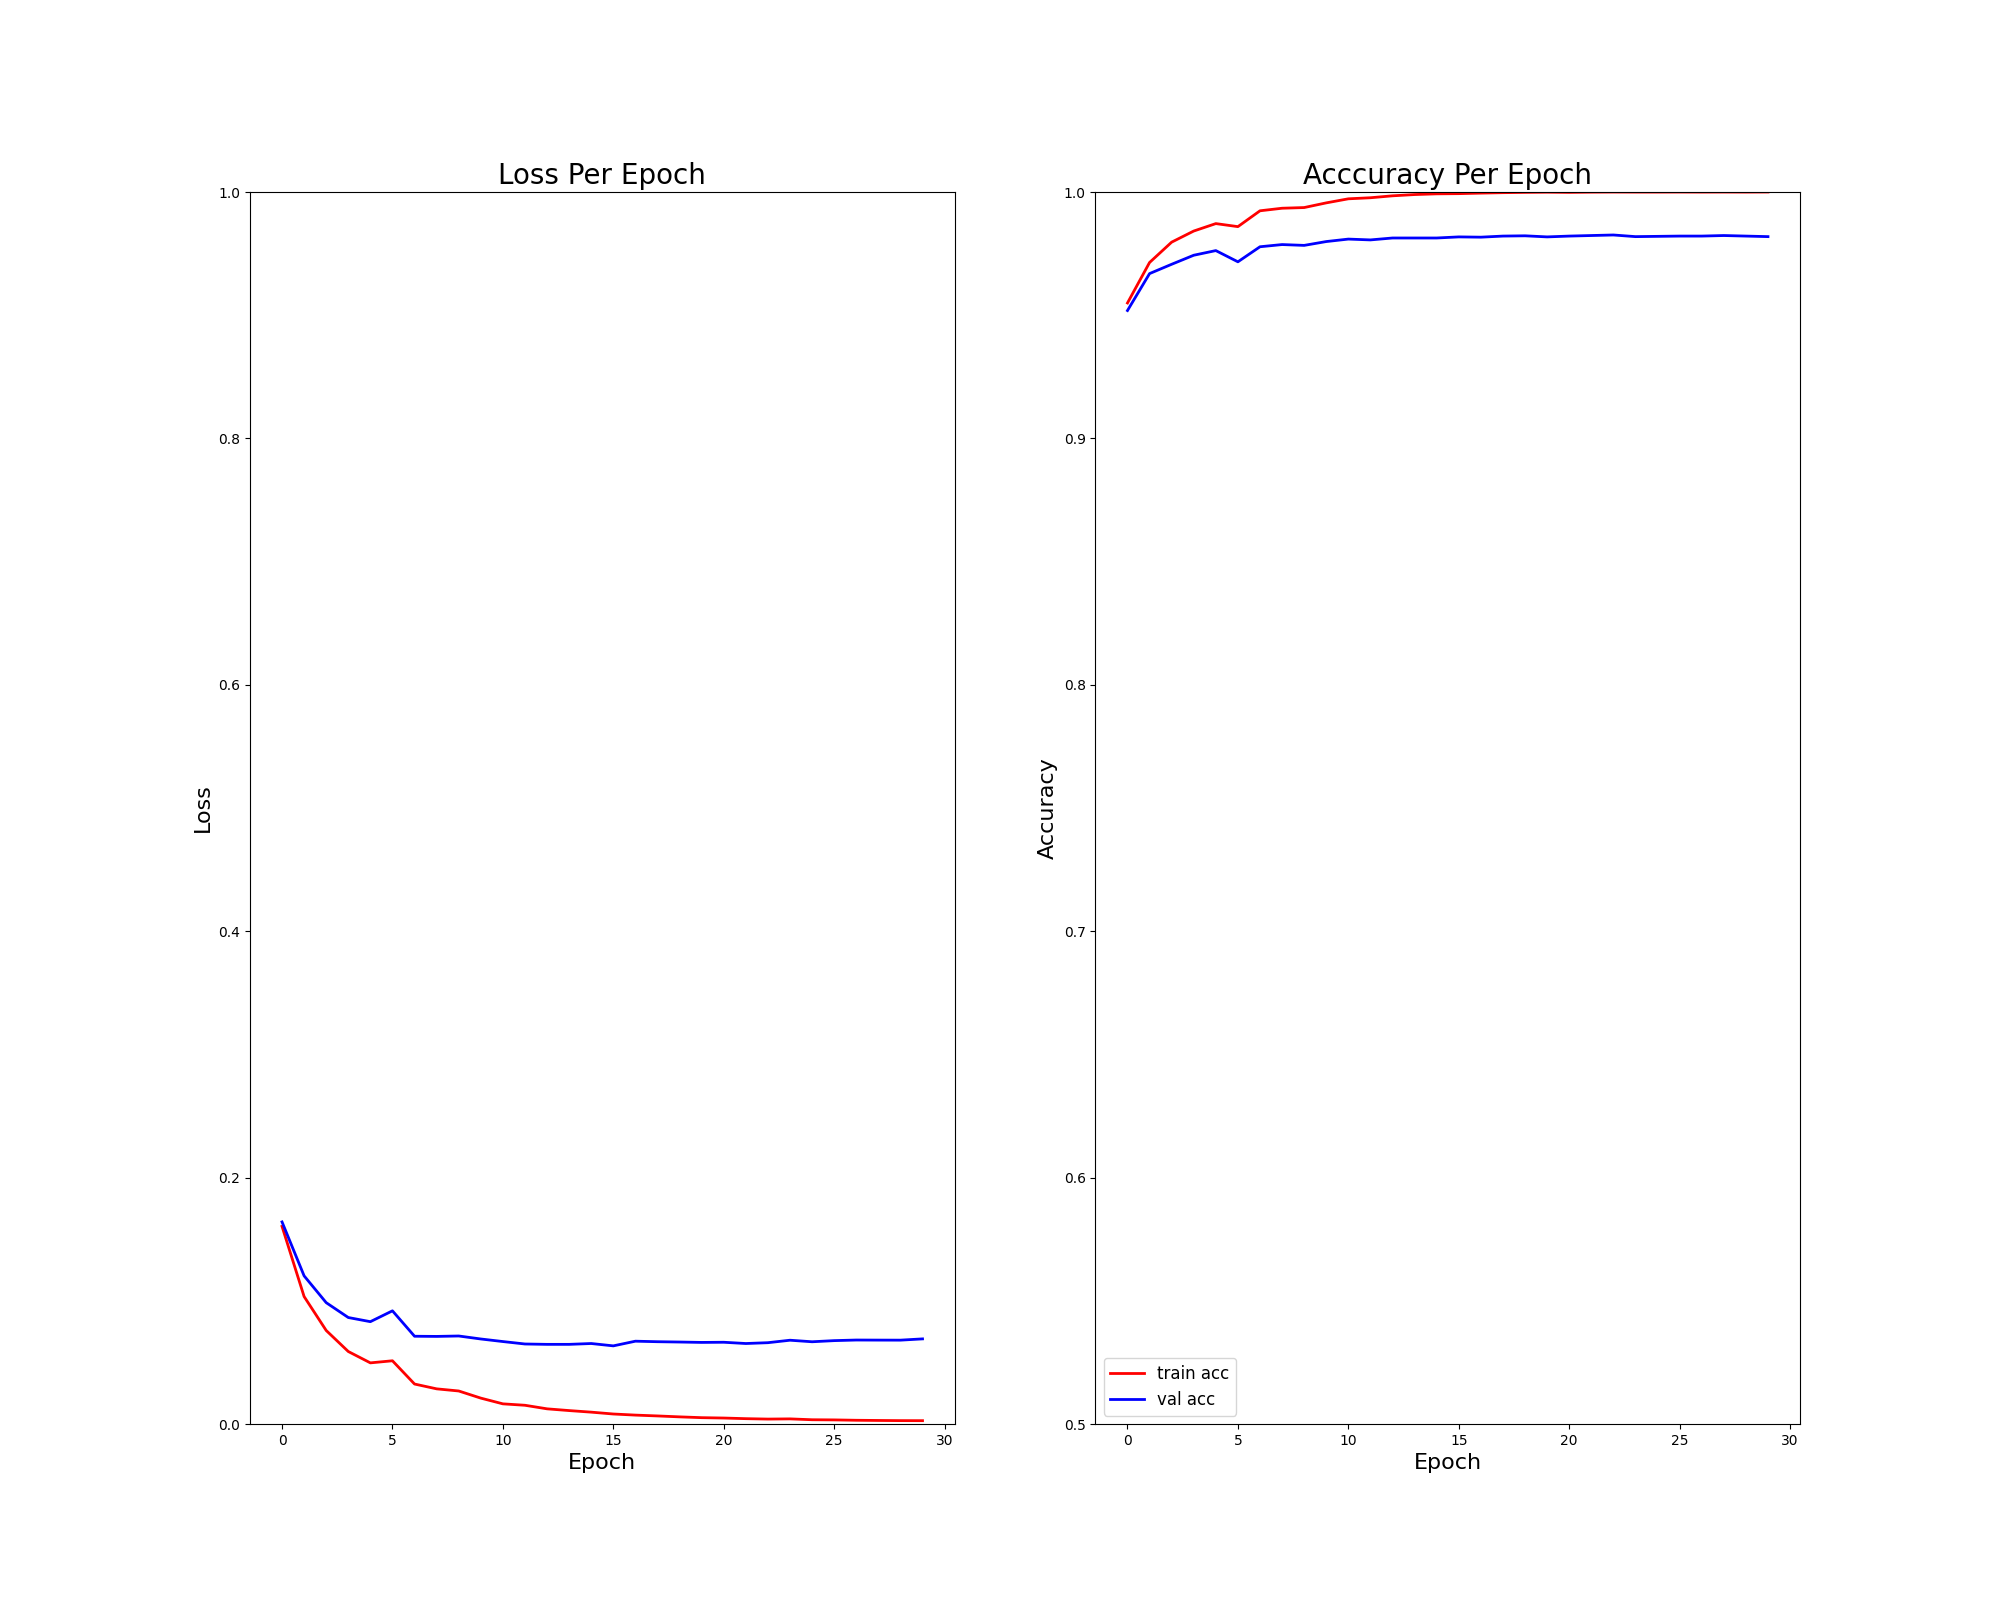
\includegraphics[width=1\linewidth]{h2_starter_code/results/epoch_plots}
		\caption{Train and validation data plots}
		\label{fig:epochplots}
	\end{figure}
	
\end{document}